%  The following commands have been added in the SPIE class 
%  file (spie.cls) and will not be understood in other classes:
%  \supit{}, \authorinfo{}, \skiplinehalf, \keywords{}
%  The bibliography style file is called spiebib.bst, 
%  which replaces the standard style unstr.bst.  
\documentclass[]{spie}  %>>> use for US letter paper
%%\documentclass[a4paper]{spie}  %>>> use this instead for A4 paper
%%\documentclass[nocompress]{spie}  %>>> to avoid compression of citations
%% \addtolength{\voffset}{9mm}   %>>> moves text field down
%% \renewcommand{\baselinestretch}{1.65}   %>>> 1.65 for double spacing, 1.25 for 1.5 spacing 
%  The following command loads a graphics package to include images 
%  in the document. It may be necessary to specify a DVI driver option,
%  e.g., [dvips], but that may be inappropriate for some LaTeX 
%  installations. 
\usepackage[]{graphicx}
\usepackage{longtable}
\usepackage{subfig}
\usepackage{lscape}
\usepackage{booktabs}
\usepackage{multirow}

\title{High Performance Si Immersion Gratings Patterned with Electron Beam Lithography} 

%>>>> The author is responsible for formatting the 
%  author list and their institutions.  Use  \skiplinehalf 
%  to separate author list from addresses and between each address.
%  The correspondence between each author and his/her address
%  can be indicated with a superscript in italics, 
%  which is easily obtained with \supit{}.

\author{Michael Gully-Santiago\supit{a}, Daniel T. Jaffe\supit{a}, Dan Wilson\supit{b}, Richard Muller\supit{b}
\skiplinehalf
\supit{a}University of Texas at Austin Department of Astronomy, 2515 Speedway St, Austin, TX, USA; \\
\supit{b}NASA JPL Microdevices Lab, 4800 Oak Grove Dr, Pasadena, CA, USA
}

%>>>> Further information about the authors, other than their 
%  institution and addresses, should be included as a footnote, 
%  which is facilitated by the \authorinfo{} command.

\authorinfo{Further author information: (Send correspondence to M.G.S)\\M.G.S: E-mail: gully@astro.as.utexas.edu}
%%>>>> when using amstex, you need to use @@ instead of @
 

%%%%%%%%%%%%%%%%%%%%%%%%%%%%%%%%%%%%%%%%%%%%%%%%%%%%%%%%%%%%% 
%>>>> uncomment following for page numbers
% \pagestyle{plain}    
%>>>> uncomment following to start page numbering at 301 
%\setcounter{page}{301} 
 

\begin{document} 
  \maketitle 

%%%%%%%%%%%%%%%%%%%%%%%%%%%%%%%%%%%%%%%%%%%%%%%%%%%%%%%%%%%%% 
\begin{abstract}
Infrared spectrographs employing silicon immersion gratings can be significantly more compact than spectrographs using front-surface gratings.  The Si gratings also offer the possibility of continuous wavelength coverage at high spectral resolution.  The grooves in Si gratings are made with semiconductor lithography techniques, to date almost entirely using contact mask photolithography.  Planned near-infrared astronomical spectrographs can require either finer groove pitches or higher positional accuracy than can be achieved with standard UV contact mask photolithography.  A collaboration between the University of Texas at Austin Silicon Diffractive Optics Group and the NASA JPL Microdevices Lab has experimented with direct writing silicon immersion grating grooves with electron beam lithography.  The device production process involves depositing positive e-beam resist on 1 to 30 mm thick, 100 mm diameter monolithic crystalline silicon substrates.  The JEOL 9300FS e-beam writer uses a 50 nm step size with a typical spot size of 300 nm at about 60 nA of current and 100 keV power.  Our typical groove frequency for echelle grating prototypes is in the vicinity of 40 $-$ 12.5 grooves/mm (25-80 $\mu$m groove spacing) but groove frequencies as high as 1000 grooves/mm are possible.  Experimental pattern sizes are up to 80 $\times$ 30 mm$^2$, but could exceed 200 $\times$ 200 mm$^2$.

There are three key challenges to produce high-performance e-beam written silicon immersion gratings.  (1) E-beam field and subfield stitching boundaries cause periodic cross-hatch structures along the grating grooves.   The structures manifest themselves as spectral and spatial dimension ghosts in the diffraction limited point spread function (PSF) of the diffraction grating.  In this paper, we show that the effects of e-beam field boundaries must be mitigated.  We have significantly reduced ghost power with only minor increases in write time by using four or more reticles of less than 500 $\mu$m. (2) The finite e-beam stage drift and run-out error cause large-scale structure in the wavefront error.  We deal with this problem by applying a mark detection loop to check for and correct out minuscule stage drifts.  We measure the level and direction of stage drift and show that mark detection reduces peak-to-valley wavefront error by a factor of 5. (3) The serial write process for typical gratings yields write times of about 24 hours- this makes prototyping costly.  We discuss work with negative e-beam resist to reduce the fill factor of exposure, and therefore limit the exposure time.
We also discuss the tradeoffs of long write-time serial write processes like e-beam with UV photomask lithography.  We show the results of experiments on small pattern size prototypes on Silicon wafers.  Current prototypes now exceed 30 dB of suppression on spectral and spatial dimension ghosts compared to monochromatic spectral purity measurements of the backside of Si echelle gratings in reflection at 632 nm.  We perform interferometry at 632 nm in reflection with a 25 mm circular beam, projected to 25 $\times$ 80 mm on the grating surface for a blaze angle of 71.6$^\circ$.  The measured wavefront error (tilt and focus removed) is 0.17 waves peak to valley.
\end{abstract}

%>>>> Include a list of keywords after the abstract 

\keywords{Gratings, Metrology, Electron Beam, Lithography, Optical devices}

%%%%%%%%%%%%%%%%%%%%%%%%%%%%%%%%%%%%%%%%%%%%%%%%%%%%%%%%%%%%%
\section{INTRODUCTION}
\label{sec:intro}  % \label{} allows reference to this section

At the last SPIE meeting we described the detailed performance of the solitary immersion grating (part number CA-1a \cite{2012SPIE.8450E..2SG}) for the high resolution infrared spectrograph IGRINS \cite{2010SPIE.7735E..54Y}.  IGRINS saw first light at McDonald Observatory on March 15, 2014.  Papers describing its performance appear in the current volume.  The technical readiness of the immersion grating now rests on firm footing, and our group has now moved on to pushing the performance and design limitations of silicon optics.  The key limitation is the immersion grating phase coherence.  Phase coherence for a diffraction grating is the extent to which repeated grating facets are positioned to the an integer value of $\sigma$, the groove constant (the desired constant spacing from groove to groove).  Specifically, the position, $x$ of the $n^{th}$ facet in a sequence of $N$ total facets is distributed as: 

\begin{eqnarray}
x_n = n\sigma + \epsilon_n  \label{eqn:Epsilon}
\end{eqnarray}

where $\epsilon_n$ is the position error for facet $n$.  Discussion of the phase performance can be broadly separated by the correlations  of errors, $\epsilon_n$, and their impact on the monochromatic spectral purity.  


There are large scale, smooth correlations:
\begin{eqnarray}
\epsilon_n = \epsilon_n(x, y) \label{eqn:smooth}
\end{eqnarray}
These errors manifest as low order optical aberrations and degrade the PSF and Strehl.  Operationally these smooth errors are the first $M$ Zernike polynomials, where $M < 200$.  There is the especially pernicious repetitive error:
\begin{eqnarray}
\epsilon_n = A\sin{\frac{2\pi n\sigma}{P} - \phi} \label{eqn:Periodic}
\end{eqnarray}
where $n\sigma$ is the desired position of the $n^{th}$ groove, $A$ is the amplitude of the error (e.g. in nm), and $P$ is the period of the error (e.g. in mm).  These errors manifest as sidelobes of the PSF called Rowland ghosts.  Although we have listed a single harmonic periodic error, any periodic structure can be broken into its Fourier components, so each of these Fourier components will be affiliated with a sidelobe Rowland ghost.  Lastly there are small scale random errors:
\begin{eqnarray}
\epsilon_n \sim \mathcal{N}(0, \sigma)
\end{eqnarray}
where $ \sim \mathcal{N}(0, \sigma)$ denotes that the error is normally distributed with mean zero and standard deviation $\sigma$.  This last type of error produces so-called spectral grass\cite{2007ApOpt..46.3400M}, which is scattered light filling the blaze.


\section{On-sky performance of Si immersion grating}
IGRINS \cite{2010SPIE.7735E..54Y} is a high resolution near-infrared astronomical spectrograph.  It employs an immersion grating as its primary dispersive element, and two cryogenic VPH gratings for cross-dispersion.  The instrument covers a wavelength range of 1.5$-$2.5 $\mu$m in two channels, namely the $H$ and $K$ atmospheric windows.  The design and early performance of IGRINS is described in this volume [talk 9147-48]\cite{2014SPIE.CHANPARK.IGRINS}.  The immersion grating for IGRINS is internal part number CA-1a.  Its lab-measured performance is summarized in Gully-Santiago et al. 2012\cite{2012SPIE.8450E..2SG}.  In this section we briefly summarize the performance of the immersion grating on-sky.

The immersion grating is performing as specified.  IGRINS has no measured performance limitation attributable to the immersion grating.  CA-1a is diffraction limited.  CA-1a has been thermally cycled about 6 times at the time of writing, with no perceptible degradation in performance.  We expect no degradation from thermal cycling.  We have previously constrained the CA-1a blaze angle to $\delta = 71.5\pm 0.2^\circ$.  In principle, we can improve our constraint on the delivered grating blaze angle from the observed echellogram.  This calculation has not been performed.

One major open question is whether CA-1a meets its spectral ghost level specification.  Spectral ghosts are secondary images which arise from periodic facet positioning errors\cite{2007sdf..book.....J}. The ghosts in CA-1a where introduced from a cyclically varying position-dependent exposure dose in the UV photolithography patterning step.  The processing error causing the ghosts has since been eliminated.  As a result our most recent immersion grating prototypes show a dramatic reduction in spectral ghosts [this volume, talk number 9151-35]\cite{2014SPIE.BROOKS.GRATINGS}.  Spectral ghosts are distributed as \ref{eqn:Periodic}.  We address spectral ghosts arising from e-beam lithography in Sections \ref{sec:Field}, \ref{sec:Boundaries}, and  \ref{sec:Ghosts}.  The ghost level depends on the amplitude of the error (cf. Equation 14 of Marsh et al. 2007\cite{2007ApOpt..46.3400M}):
\begin{eqnarray}
	\frac{I_g}{I_0}=[ \frac{2\pi n}{\lambda}A \sin{\delta} ]^2	 \label{eqn:GLevel}
\end{eqnarray}
where $I_g/I_0$ is the ghost level relative to the main peak, $\lambda/n$ is the wavelength scaled in the refractive index, and $A$ is defined in Equation \ref{eqn:Periodic}.  We predicted an in-immersion ghost level of $I_g/I_0 \sim2\times10^{-3}$ at 1.5 $\mu$m based on visible laser metrology\cite{2012SPIE.8450E..2SG}.  At the time of writing the IGRINS commissioning team has constrained ghost levels at $\lambda=1.5 \; \mu$m to $I_g/I_0 < 1\times10^{-2}$.


\section{Motivations for direct writing Si immersion gratings}
There are a few key motivations for adopting e-beam direct writing over conventional contact photolithography.  

\subsection{Higher precision than contact lithography}
\label{sec:Precis}
Electron beam lithography is more precise than contact lithography.  The figure of merit for precision in e-beam lithography is the so called \emph{spot size}, the typical diameter of the e-beam pulse at the location of the e-beam sensitive resist on the substrate surface.  E-beam spot sizes on the JEOL 9300FS tool can be as low as 2 nm.  Admittedly the e-beam current at a 2 nm spot size is prohibitively low.  In practice, a 200 nm spot size is used.  The final precision is a small fraction of the spot size, since many adjacent spots are convolved together.  In later sections we directly compare the performance of immersion gratings produced with e-beam and contact lithography to show evidence that we have achieved much higher precision in e-beam lithography.  

\subsection{Finer groove pitch capability than contact lithography}
Owing to its small achievable spot size, electron beam lithography can reach finer groove spacings than contact photolithography can.  Fine pitches are required for high dispersion in low order.  Our groups are currently designing a fine ($\sigma \; \sim$ 2 $\mu$m) pitch pattern immersion grating for the NASA Earth Science Technology Office (ESTO) Advanced Component Technologies (ACT) program.  The ACT mission concept requires high spectral resolution at low order ($\sim1-10$).  The grating pattern designs employing first or second diffraction order cannot be made with contact lithography.  Higher order devices can be made with contact lithography, but suffer from order overlap and reduced bandwidth.  The reduced bandwidth limits conceivable designs to less than about $16^{th}$ order.  The combined background at high order overlap is a concern.  For a narrow band filter with 0.1\% off-band rejection, we can expect to see up to 1\% background level.  A first order grating with fine pitch eliminates the need for narrow band filtration, and should achieve much lower than 1\% background levels.  


\section{e-beam patterning strategies}
This section explains the e-beam patterning strategies.  Specifically, we explain in detail the hierarchy of e-beam patterning geometries.  The relationships of these geometries affect the relative power distributed among spectral and spatial scales in the delivered monochromatic PSF.

\subsection{e-beam patterning geometry hierarchy}

\begin{figure}
\begin{center}
 \begin{tabular}{c}
    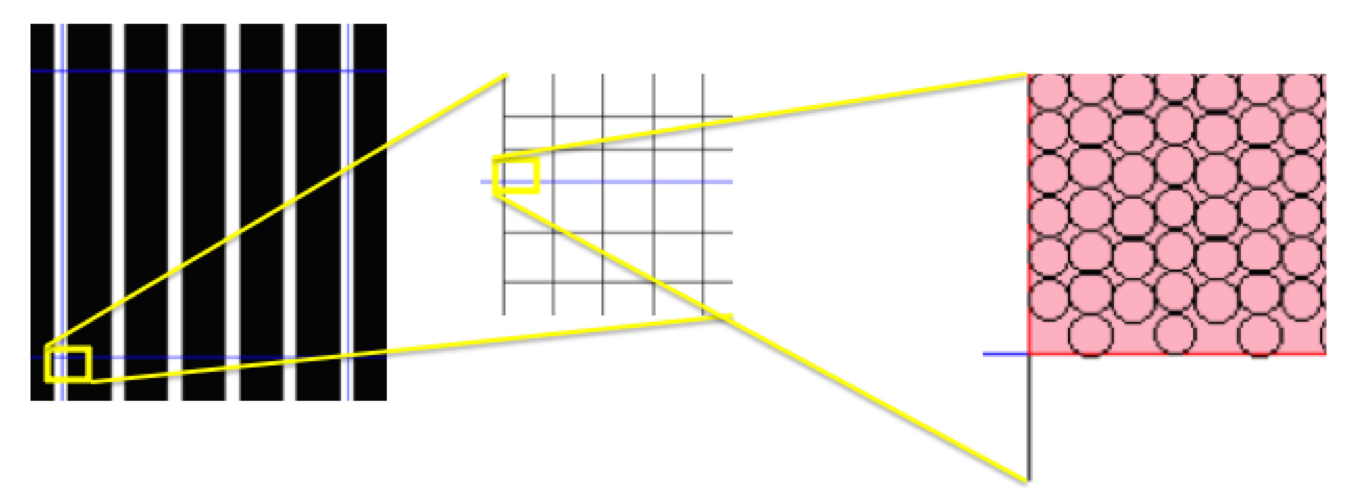
\includegraphics[width=0.8\textwidth]{figs/Field_sizes_cascade_02.png}
   \end{tabular}
  \end{center}
  \caption[e-beam Hierarchy]{\label{fig:Hierarchy} Hierarchy of e-beam geometries- in the left panel the grooves are black and the fields are thin blue lines, the middle inset shows subfields, and the right inset shows spots at a regular step spacing, though the spots are not to scale.  Spot sizes are typically about 4-5 times their spacing.}
\end{figure}


There are five key geometries in e-beam lithography.  These geometries are typical among e-beam tools, though we focus our discussion to the geometries relevant to the JEOL 9300FS.  The geometries in order of small to large scales are step size, spot size, subfield deflector size, field deflector size, and stage range of motion.  The largest scale geometry- the stage range of motion- simply limits the maximum pattern size, so we do not discuss it in detail in this subsection.  Figure \ref{fig:Hierarchy} shows a cartoon of the hierarchy from left to right- field, subfields, and spots.

\subsubsection{e-beam step size and spot size}
The e-beam step size is the center-to-center separation of the e-beam spots.  In an analogy to a jackhammer, the step size is the spacing between punctures of asphalt.  Step sizes can range from roughly 2 to hundreds of nanometers.  We adopted a 50 nm step size for our immersion grating patterns.  The rationale for the step size depends on understanding the e-beam spot size.  

The spot size controls the smallest achievable feature size, as alluded to in Section \ref{sec:Precis}.  Our spot size was between $150-300$ nm, but typically about 230 nm.  Several operational properties of the electron-beam gun affect the spot size, so we mention those here for clarity.  The e-beam gun focuses fast-moving electrons to a spot.  The spot size can be decreased by preferentially removing those electrons with large velocity components perpendicular to the bulk direction of motion.  This preferential removal of fast electrons is achieved with a grounded conductive circular aperture somewhere in the beam path prior to the spot formation.  The aperture is constricted to reduce the spot size.  The net current (e$^-$/s) consequently decreases, since the aperture has effectively thrown away electrons.  So there is a tradeoff between current and spot size.  This tradeoff is important in deciding optimal patterning strategies and sizes.  Our choice of a relatively large spot size ($\sim 200$ nm) came from the economical need to limit the expensive e-beam write time, with the understanding that the spot size is small enough to achieve the specified precision of $< 25$ nm.

The conductive aperture setting coarsely selects the range of spot size achievable, while the detailed spot size depends on fine adjustments made to the e-beam column before an exposure.  These adjustments are familiar for those who have used scanning electron microscopy- astigmatism, wobble, and focus, for example.  Poor calibration might deliver an elliptical, asymmetric spot shape.  In practice, a slightly asymmetric spot shape does not affect the performance of immersion gratings.

A key idea is that the step size (50 nm) is much smaller than the spot size ($\sim200$ nm) so that adjacent steps convolve to form a fairly uniform exposure area.  Another key assumption is that the e-beam spot does not change significantly over the course of an exposure.  We expect that the e-beam spot is unchanged, so long as the e-beam column is unperturbed.

\subsubsection{Subfield deflector}
The subfield deflector is a component of the e-beam gun that minutely redirects the e-beam spot within a box of up to 4 $\mu$m edge, centered around a mean position set by the main field deflector.  Table \ref{tab:D07andE12} lists the subfield sizes for parts D07 and E12.  For example we chose subfield sizes of 3.7 and 2.9 nm for D07 and E12, respectively.  For recent work on fine pitch ($\sim2\; \mu$m) gratings we have experimented with smaller subfield sizes.  For perspective, the choice of subfield size of $4 \; \mu$m square has 80 $\times$ 80 steps of 50 nm. 

\subsubsection{Field deflector}
\label{sec:Field}
The field deflector, also sometimes called the main-field deflector, coarsely redirects the electron beam up to a 500 $\mu$m square.  The main-field deflector can be thought as positioning the center of the subfields.  For example, the choice of a 500 $\mu$m square field size and 4 $\mu$m square field size would result in 125 $\times$ 125 subfields.

The fields are stepped together by the interferometrically controlled stage.  Once an entire field's pattern has been written, the stage steps to the next adjacent field to write.  The stage move speed is typically much slower than the field and subfield deflector speed, so small field sizes are inefficient in time-on-target compared to wall-clock time.  The performance of the field deflector degrades with distance from the center (e.g. pincushion distortion), so there is a tradeoff between write speed and performance.  

The choice of field size is multifaceted.  Field size choice is one of the key strategies for mitigation of ghosts.  We address the issue of field size choice in detail in Section \ref{sec:Ghosts}.  

\begin{figure}
\begin{center}
 \begin{tabular}{c}
    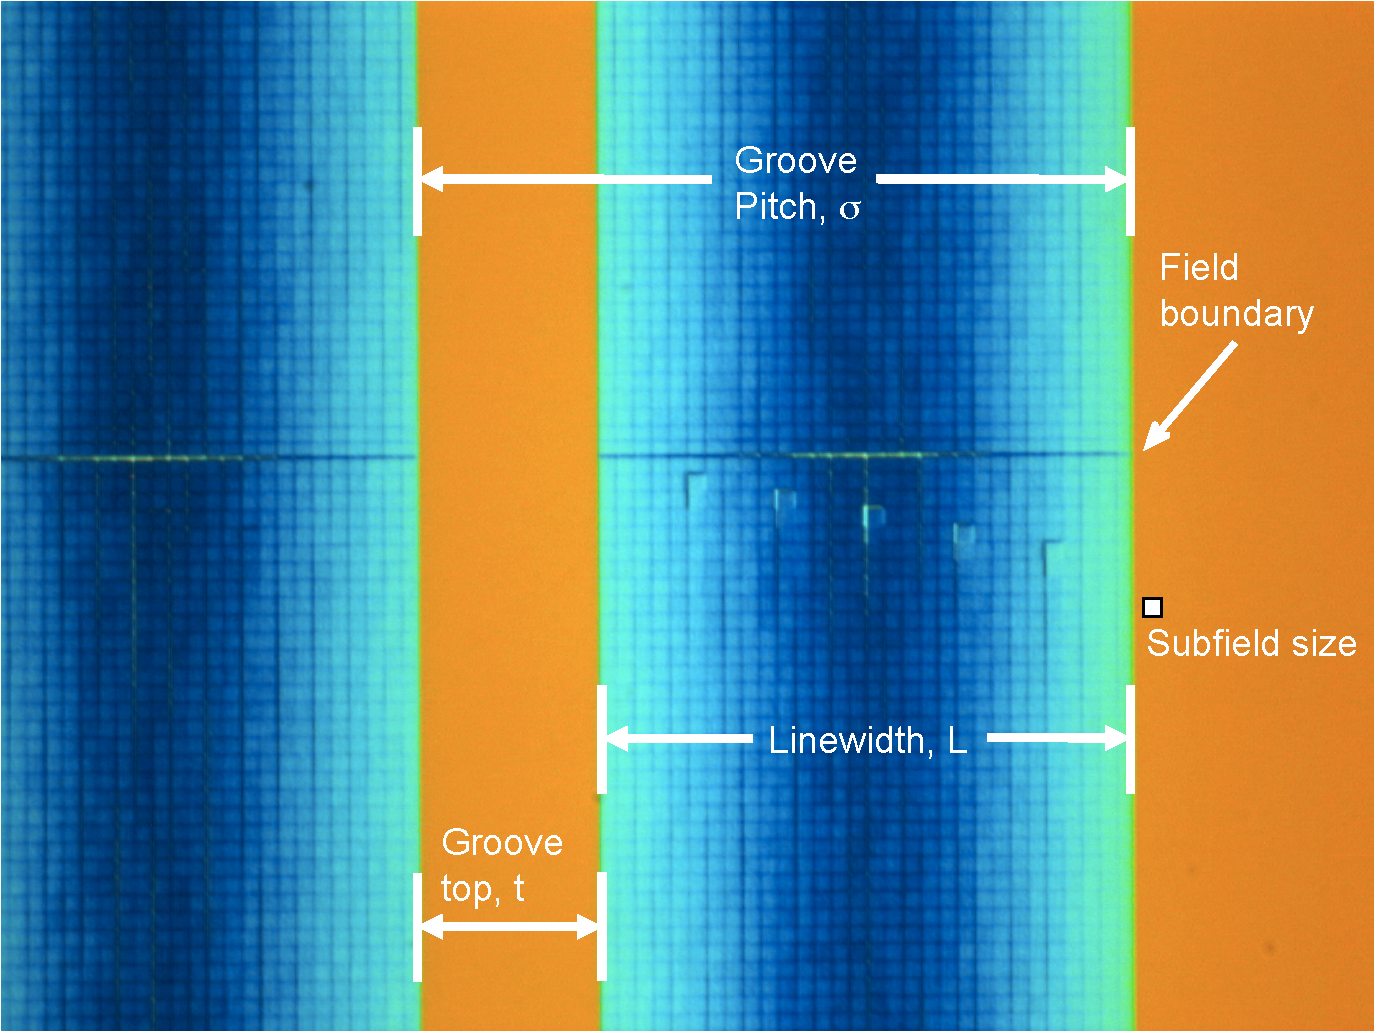
\includegraphics[width=0.96\textwidth]{figs/subfields_TJ04_Zeiss.pdf}
   \end{tabular}
  \end{center}
  \caption[TJ04 under Zeiss]{\label{fig:TJ04Zeiss} Subfield and field boundaries directly perceptible in optical microscopy of the e-beam resist on an intentionally underexposed sample, TJ04.  The groove pitch for this sample is 100 $\mu$m, with a 75 $\mu$m written linewidth.  The blue area is the linewidth portion of the grating which has e-beam resist already exposed to e-beam.  The orange line is the groove top, where the e-beam resist was unexposed and would have served as the wet etch dam, had the linewidth actually developed out.  The minute color differences within the exposed linewidth are attributable to tiny thickness differences of the resist, which originate from tiny differences in delivered e-beam dose.  The cylindrically symmetric color difference of teal to dark blue is attributable to the proximity effect as described elsewhere\cite{2005SPIE.5720...68W}.  The tiny boxes are subfields, which are only perceptible due to subtle subfield stitching errors.  Some fields are more errant than others.  The thick horizontal stripe is a portion of a much larger field boundary, perceptible only because of main-field deflector stitching boundaries as discussed in the text.}
\end{figure}

\subsubsection{Interplay of hierarchy at boundaries and design rules}
\label{sec:Boundaries}
The e-beam geometries must match up at the boundaries.  We learned many subtle design rules unique to high performance immersion gratings.  The main theme in all of the design rules is to avoid fractional steps in the writing process.  The JEOL pattern generation software inserts patterns of spaces and spots when it reaches a command for a fractional step.  The specific design rules below are probably unique to the JEOL pattern generation software.  Other e-beam tool software is likely to have different design rules.
\begin{enumerate}
  \item Subfields must be integer number of steps
  \item Fields should be integer number of subfields.  
  \item Linewidth should be an integer number of subfields.
  \item Field sizes and linewidths can be non-integer number of subfields only if the remainder fractional subfield plus one subfield divided by two is an integer number of step sizes.
\end{enumerate}   

These rules ensure that all e-beam spots are equidistant.  Figure \ref{fig:Hierarchy}  shows the JEOL \emph{shot shape display} which broke rule 2 and 4.  Metrology of a grating prototype that broke rule 2 and 4 resulted in unacceptably large grating ghosts in the cross-dispersion direction.  The line-edge of contiguous spots lacked a solitary spot near the subfield boundary.  Such a periodic dearth in exposure manifested as a periodic divot along the length of the groove.  The detailed impact on optical phase depends on the relative step size, e-beam sensitive resist contrast, and sundry subsequent processing steps.  Rather than risk a performance degradation it is best practice to avoid the formation of subfield blips in the first place.  The main concern for a final application is probably scattered light, and not efficiency loss. 


\begin{table}
	\begin{center}
	\caption{D07 and E12 e-beam pattern details. \label{tab:D07andE12}}
	\begin{tabular}{ccc}
	\toprule
	   &D07 & E12  \\
	\midrule
	substrate bias angle ($^\circ$) & 6.1 & 71.5 \\
	pattern size (mm) & 39.0 x 39.664 & 29.696 x 84.816 \\
	pitch ($\mu$m) & 7.8 & 27.36 \\
	top width ($\mu$m) & 0.4 & 9.96 \\
	line width ($\mu$m) & 7.4 & 17.40 \\
	step size (nm) & 50 & 50 \\
	steps per linewidth & 148 & 348 \\
	subfield size ($\mu$m) & 3.7 & 2.9 \\
	subfields per linewidth & 2 & 6 \\
	steps per subfield & 74 & 58 \\
	\cline{1-1}
	 			      & 63: 491.4  & 17: 465.12 \\
	grooves per $x-$field and & 61: 475.8 & 15: 410.4 \\
	$x-$field sizes ($\mu$m) & 59: 460.2 & 13: 355.68 \\
	 				        & 55: 429.0 & 11: 300.96 \\
	\cline{1-1}					        
	 			      & 134: 495.8  &   \\
	subfields per $y-$field and & 133: 492.1 &   \\
	$y-$field sizes ($\mu$m) & 131: 484.7 & 160: 464.0 \\
	 				        & 127: 469.9 &   \\	
	\cline{1-1}
	\bottomrule
	\end{tabular}
	\end{center}
\end{table}	



\subsection{Predicting the ghost level associated with field positioning errors}
\label{sec:Ghosts}

The field size is only a few times larger than our typical coarse echelle grating groove constants.  Figure \ref{fig:FieldCartoon} shows an exaggerated cartoon of the field size relative to grooves.  In a hypothetically perfect e-beam field stitch, the line positions are exactly as desired.  In reality there is some finite distortion, which is repeated each time the field is written into the e-beam resist.  We define the ratio, $G$, as the field size, $F$, divided by the groove pitch size, $\sigma$.  For example, let's say we have a field size $F\;=\;500\;\mu$m and a groove constant $\sigma \; =\; 100 \; \mu$m.  Then $G\;=\;5$.  So there will be 5 grooves per field.  The omnipresent field deformations will be rubber stamped into each field, repeating every 5 grooves.  The cyclically varying facet positions manifest as ghosts with G-fold symmetry. We expect $G-1$ inter-order ghosts, separated by a fraction $1/G$ of the inter-order separation.  For the $G\;=\;5$ example, there are 4 inter order ghosts, separated by a fifth of the order angular separation.  In Section \ref{sec:MultipleFields} we describe our strategy for mitigating power by distributing the power into multiple fields.


\begin{figure}
\begin{center}
 \begin{tabular}{c}
    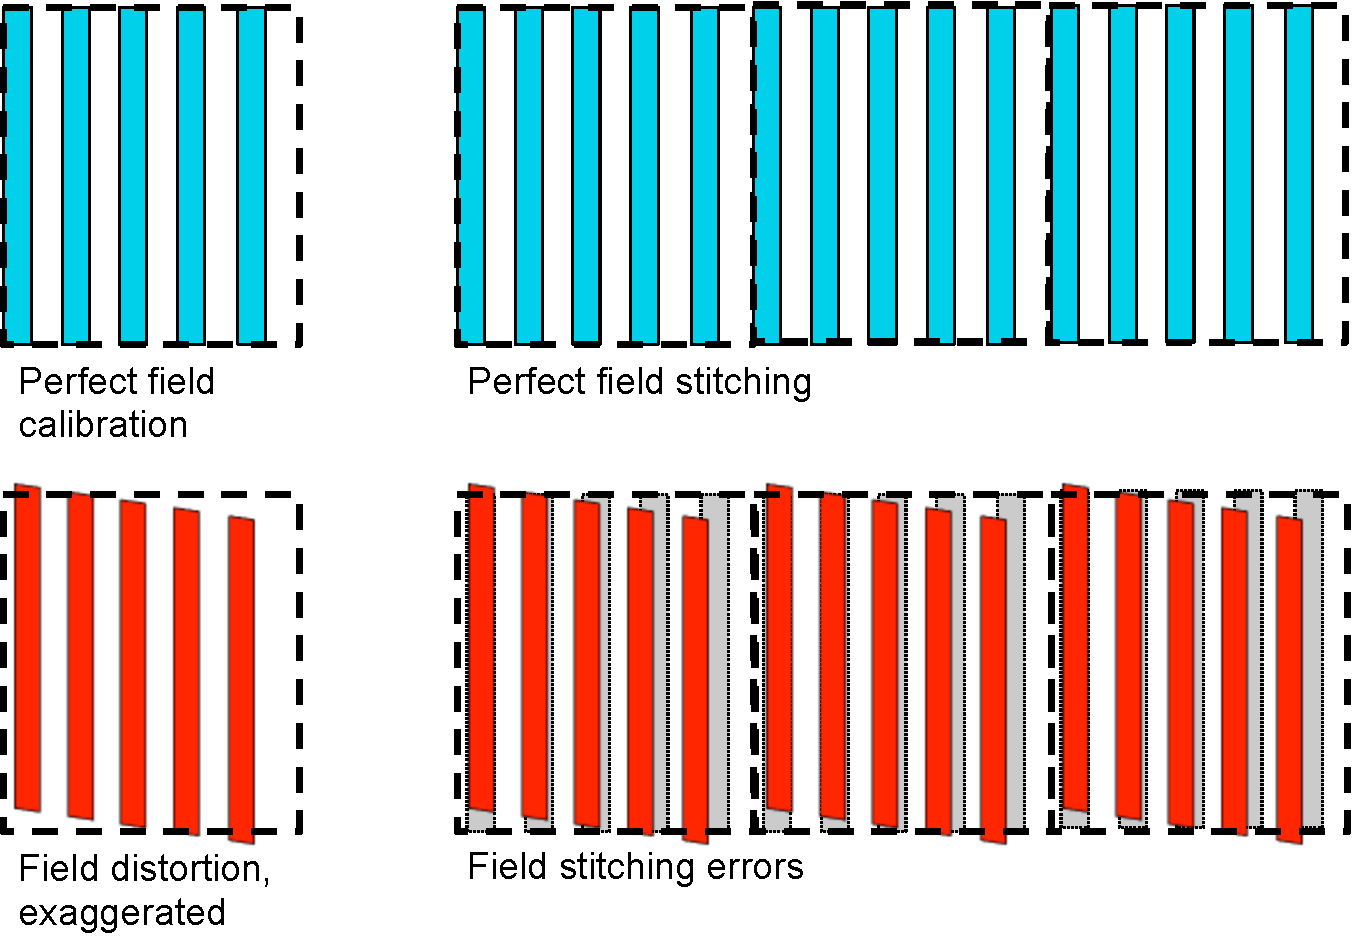
\includegraphics[width=0.6\textwidth]{figs/Field_stitching_errors.pdf}
   \end{tabular}
  \end{center}
  \caption[Field Stitching Error Cartoon]{\label{fig:FieldCartoon} An exaggerated cartoon to demonstrate the repetitive nature of field stitching.  A typical field size is about 300-500 $\mu$m on a side, and typical groove periods, $\sigma$, are about 20-100 $\mu$m.  There are only a few to tens of grooves per field.  The distortion shown in the cartoon is highly exaggerated, and in reality the calibration is much better than depicted.  Additionally, the morphology of the distortion is not well characterized.  We have depicted a parallelogram shape, though the realized morphology could be more like pincushion or barrel distortion.  The fields could also be perfectly square and simply misplaced in their center positions, still causing errors.  The details of the morphology might give rise to differing relative levels of harmonics, in a Fourier sense.  To put the scale in perspective, we coarsely estimate the repetitive position error amplitude A (cf. eq. \ref{eqn:Periodic}) as about 5-50 nm from experiments on e-beam wafers.  Compare this minuscule position error with the $\sim500 \; \mu$m field size, to see that the fractional position error is 1 part in $10^4$ or better.}
\end{figure}

In principle it is possible to predict the ghost levels relative to the main diffraction peak with some information about the magnitude and shape of the field distortion.  For example, in the limit of perfect field positioning (i.e. with identically zero error, $\epsilon_n(x,y)$), then there are no grating ghosts.  As the amplitude of the field distortion is dialed up, the grating ghost level increases approximately as Equation \ref{eqn:GLevel}.  In practice, we have not directly measured the field distortion, which we expect to be a function of both $x $ and $y$.  We have measured the ghost levels, and report them in Section \ref{sec:MeasGhost}.

\subsection{Employ multiple fields sizes rather than one field size}
\label{sec:MultipleFields}
In this subsection we report our main strategy for mitigating the ghosts attributable to field stitching errors.  There are two main strategies for mitigating ghosts.  One is to reduce the overall power in ghosts, using a single field size.  The other is to merely redistribute the power into different spatial scales, by using a variety of field sizes.  The strategies can be combined.

First let's address our main strategy, which is to merely redistribute the field power into several different spatial scales.  In other words, rather than use a single field size, say 500 $\mu$m, we break up the field into several fields, say 500, 450, 400, and 350 $\mu$m.  The resulting diffraction grating will have more unique inter-order ghosts, but with each ghost of lower intensity compared to ghosts attributable to a single field.

Now let's address strategies for reducing the overall power in a single field size.  One way is to select a small field size, say $F=$ 200 $\mu$m.   We know that the e-beam field performance is better in the center, and deviates towards the edge of the field.  The tradeoff with this strategy is that the stage move time is long compared to the e-beam field deflector time, so the write duration increases.  Another strategy for reducing the power in ghosts attributable to a single field size is to improve the intra-field calibration.   We could remove, for example, the minute pincushion or barrel distortion familiar from cathode ray tube computer monitors.  In practice it is tricky to measure, and therefore correct for, these minuscule distortions beyond some low residual level that we have not quantified.  

There is one key strategy that has had some success at reducing the overall power in spatial distortions of e-beam fields.  This key strategy is to experimentally determine the optimal height offset for the e-beam focus.  For whatever reason, the JEOL 9300FS selects a default writing height which is offset from the optimal height.  We experimentally verified an offset which slightly reduces the overall distortion in the fields.  We are still integrating this technique into our writing strategy at the time of writing.

Lastly, there are some slightly obscure JEOL e-beam commands relevant to ghost mitigation.  These are the ``overlay'', ``gather'', and other affiliated commands.  The main idea behind these writing strategies is to re-write over a patch of grating so that it sees different portions of the field, and therefore the field distortions average down.  We experimented with these techniques but found that they unacceptably increase the write times.

\section{Prototype immersion gratings produced with e-beam patterning}


\subsection{Measurement of ghost levels for a variety of writing strategies}
\label{sec:MeasGhost}
In Figure \ref{fig:GhostLevelFig} we show measurements of inter order ghosts for experiments TJ03 and TJ04.  Each grating received a different treatment for e-beam field geometry.  The grating pattern details are listed in Table XX.  The first result is that virtually all ghosts are below 10$^{-3}$ of the main peak.  Some ghosts were expected but not detected (denoted ND in the plot legend).  The non-detections are probably related to instrumental limitations, though upper limits are not available.  

\begin{table}
	\caption{Wafer TJ04 pattern details.  \label{tab:TJ04details}}
	\begin{tabular}{lllcccccccccc}
	\toprule
	 &   & & \multicolumn{10}{c}{Grating Area} \\
	\cmidrule(l){4-13}
	Geometry & & Unit & A  & B & C & D & E & F & G &  H &  I & J\\
	\midrule
	\multirow{2}{*}{Pattern length}& (x) & mm &  \multicolumn{10}{c}{15} \\
	 & (y) & mm & \multicolumn{10}{c}{10} \\
	Pitch && $\mu m$ & \multicolumn{6}{c |}{100} &\multicolumn{4}{c}{25}  \\
	Linewidth && $\mu m$ & \multicolumn{6}{c |}{75} & \multicolumn{4}{c}{22.5}  \\
	\multirow{2}{*}{Field}&(x) & $\mu m$ & 100 &  200 & 200 & 200 & 500 & Multi & 100 & 200 & 500 & Multi \\
	&(y)& $\mu m$ & 500 & 500 & 100 & 250 &  500 & 500 & 500 & 500 &500 & 500\\
	Subfield && $\mu m$ & 2.5 & 2.5 & 4.0 & 4.0 & 2.5 & 2.5 & 2.5 & 2.5 & 2.5 & 2.5 \\
	Spot && nm & \multicolumn{10}{c}{$\sim300$} \\
	Step && nm & \multicolumn{10}{c}{50} \\
	\bottomrule
	\end{tabular}
\end{table}

\begin{figure}
\begin{center}
 \begin{tabular}{c}
    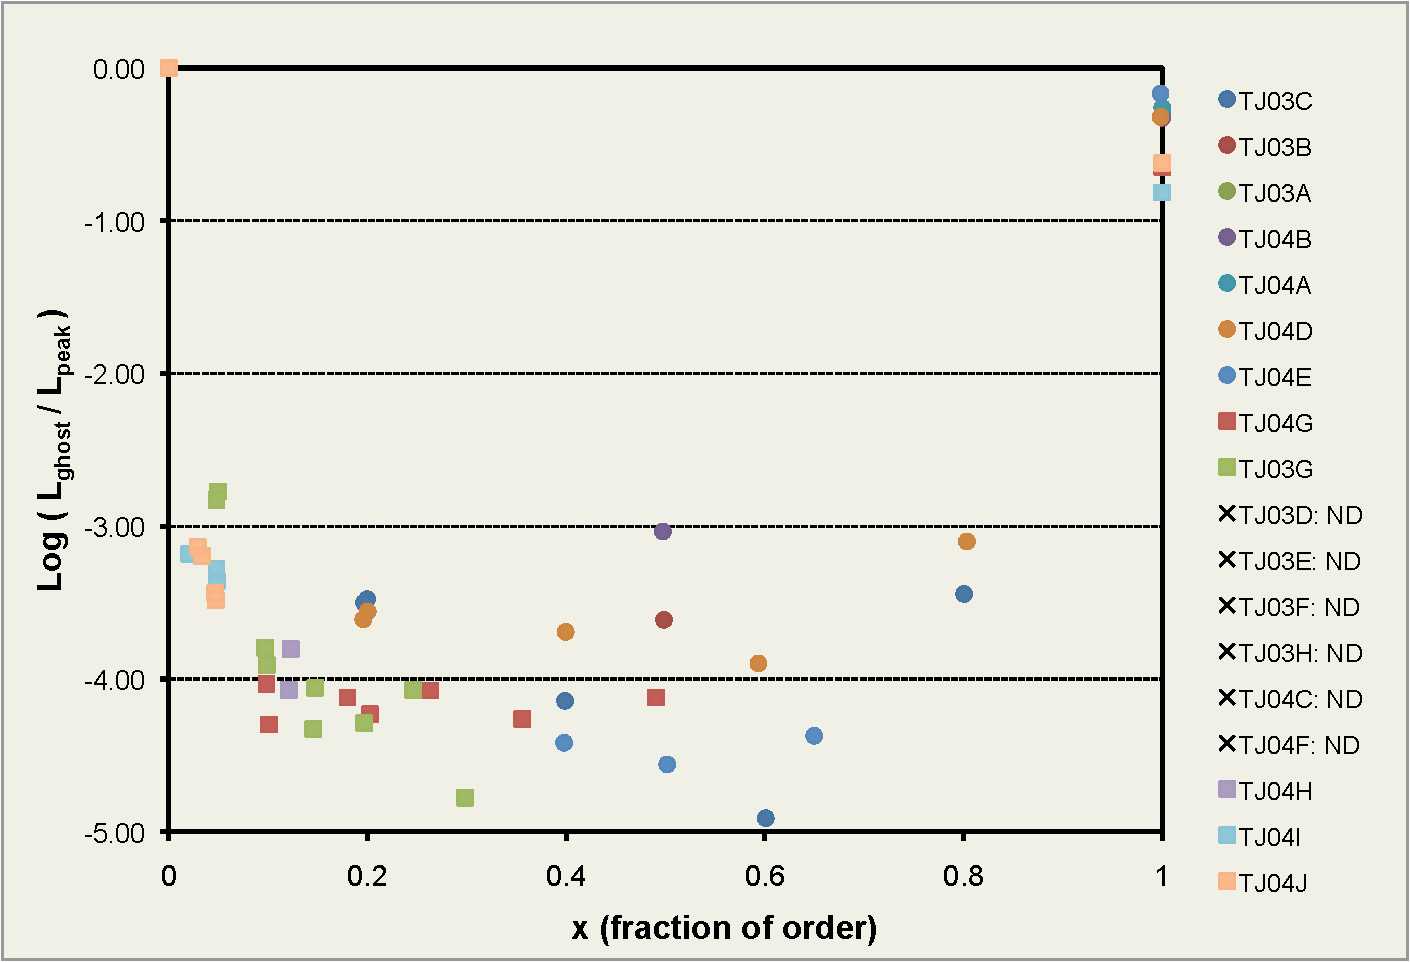
\includegraphics[width=0.8\textwidth]{figs/TJ04_ghosts_pretty_alt.pdf}
   \end{tabular}
  \end{center}
  \caption[Ghost level measurements]{\label{fig:GhostLevelFig} Measurements of the levels of inter-order ghosts for a variety of e-beam patterning strategies.  The levels are normalized to the brightest order.  A full order is shown, with the $x-$axis units normalized to an order spacing.  The grating prototype TJ04 is described in the text.}
\end{figure}

%\subsection{Is there a need for multiple cross-dispersion field sizes?}

\section{Strategies for mitigating facet position errors attributable to large scale stage drift}

One key innovation of this work is the characterization of the e-beam stage drift.  Secular drift of the e-beam stage causes large scale facet position errors which manifest as optical aberrations.  In this section we explain how to measure and correct out the e-beam stage drift.

\subsection{Characterization of e-beam stage drift}
We characterized the e-beam stage drift with built-in JEOL commands in the .JDF file.  Specifically, we used the \emph{DRIFT} and \emph{CURRENT} commands.  The \emph{DRIFT} command checks the position of the stage by scanning a gold nanoparticle mounted to the stage.  The process ties the actual position to the predicted position to the precision of the nano particle's centroid, which is a small fraction of the 200 nm spot size.  We measured a precision of about 15 nm in the centroid process.  Having determined the amplitude and direction of the drift, the \emph{DRIFT} command subtracts out the offset and continues writing with its updated coordinates.

The centroiding \emph{DRIFT} process can be automatically repeated on a desired frequency.  We set a frequency of 10 minutes.  For a typical 20 hour write we achieve 120 drift corrections.  The JEOL software logs these corrections, so we can reconstruct the path of the drift, had we not taken action to correct it.  Figure XX shows one of these reconstructions for sample E12.

\begin{figure}
\begin{center}
 \begin{tabular}{c}
    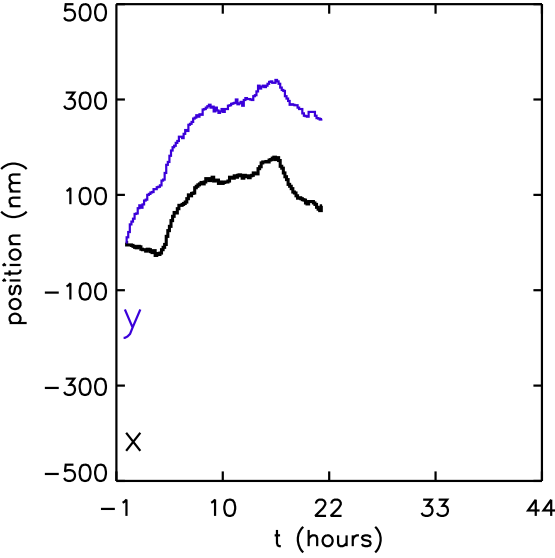
\includegraphics[width=0.4\textwidth]{figs/E12_drift_ebeam.png}
   \end{tabular}
  \end{center}
  \caption[Drift amplitude]{\label{fig:ebeamDrift} The reconstructed drift of the JEOL 9300FS e-beam stage during the patterning of sample E12.  The write time was 20.9 hours, with drift samples every 10 minutes.  The $x$ and $y$ components are separated and plotted as a function of time.  The top curve is the $y$ drift.  The curves begin at 0 at time zero, and show a range of motion of $\Delta x = $ 206 nm and $\Delta y = $ 341 nm.  This amplitude of drift would have been catastrophic for a grating which has line edge specifications of $\lambda/10 \sim 60 $ nm for diffraction limited performance in $J-$ band.  The JEOL9300FS command \emph{DRIFT} automatically corrects out this drift, so the maximum realized drift is merely the minuscule difference that occurs over the 10 minute interval between corrections.  Figure XX shows a direct comparison of prototype gratings patterned with and without drift correction.  }
\end{figure}



 We do not know the reason for differences in predicted versus realized stage position, though we can speculate.  Our best lead is that there is thermal expansion attributable to heat conduction from the warm Si puck and holder unit into the stage.  Specifically, there is some evidence that the drift rate is largest at the beginning of the writing, perhaps while thermal equilibration is still happening.  The thermal probes on the stage lend some credibility to this idea, since the probes asymptote to constant value after a few hours.  Owing to this possibility, we recommend delaying the start of a write until the sample and holder have come into thermal equilibrium with the stage.  Beyond this thermal explanation, there are many conceivable reasons why there could be drift.  At some level we do not care, as long as we can correct it out sufficiently well.  The cost of correction is merely a hit in extended write time for the same written area, i.e. a decrease in efficiency.  We found roughly a 10\% overhead associated with drift checking.

\subsection{Improvement in wavefront performance from drift correction}
In Figures \ref{fig:E09igram} and \ref{fig:E12igram} we show the dramatic impact of drift correction on the performance of our Si gratings.  The stark difference between wavefront performance with drift correction and without drift correction is the ``smoking gun'' that the e-beam must have drift correction enabled to achieve high performance diffraction limited performance.  At the time of writing we have produced and tested another immersion grating with even higher performance than E12.  We summarize the performance of e-beam produced gratings in comparison to their UV photolithographically produced counterparts in Figure XX.

\begin{figure}
   \subfloat[E12 Interferogram]{\label{fig:E12igram}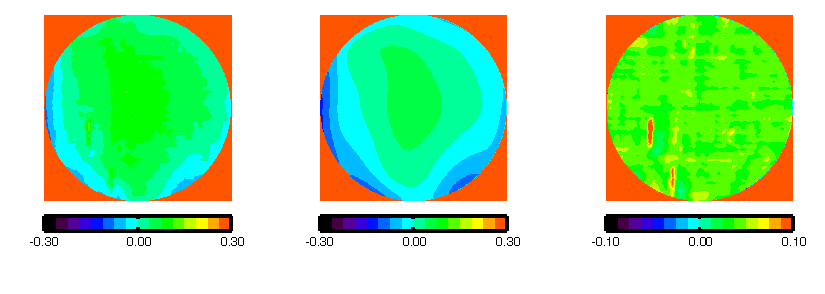
\includegraphics[height=5cm]{figs/E12_fig_scl2.pdf}}
   \newline
  \subfloat[E09 Interferogram]{\label{fig:E09igram}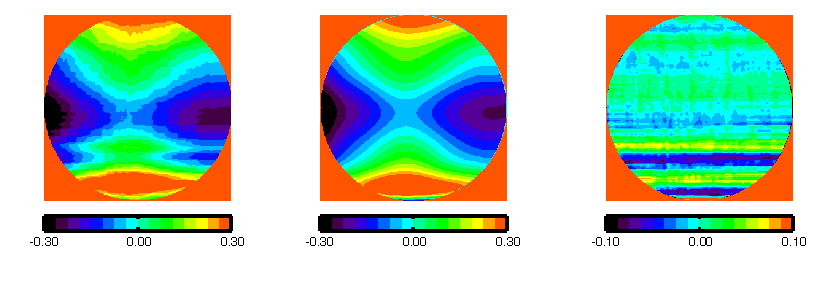
\includegraphics[height=5cm]{figs/E09_fig_scl2.pdf}}
  \caption{Comparison of immersion grating surfaces on samples E09 and E12 measured with $\lambda = 632.8 $ nm interferometry.  The color scale is reported in fractions of waves of surface deviation.  The patterns on E09 and E12 are identical: $\sigma = $ 27.36 $\mu$m, with a 9.96 $\mu$m groove top.  The groove top is not shadowed in these measurements which are taken in reflection in air, but we assume the groove tops have negligible impact on the measured interferometry.  The interferometry is performed with a 25 mm circular beam, which is projected over an 80 mm $\times$ 25 mm ellipse at the R3 echelle blaze angle, $\delta = 71.5 ^\circ$.  The left panel is the measured interferometry.  The middle panel is a decomposition into the first $\sim 80$ Zernike terms.  The right panel is the residual.  E09 was written on May 4, 2011, E12 was written September 1, 2011.  The only difference between the samples is that E09 was written with \emph{DRIFT} and \emph{CURRENT} check protocols with the JEOL e-beam writing software.  The outcome is dramatic- E12 has $\sim 4$ times lower surface deformation than E09.  Note that the vertical color bars are on the same scale to ease visual comparison.}
  \label{fig:igrams}
\end{figure}


\begin{figure}
  \begin{center}
 \begin{tabular}{c}
    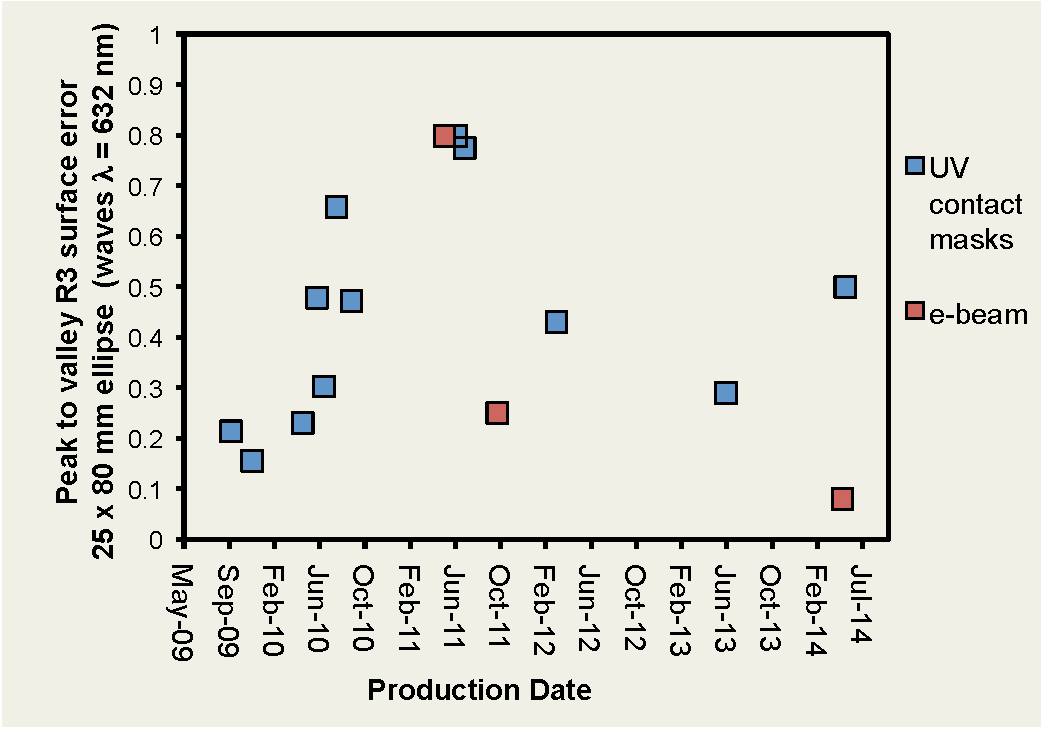
\includegraphics[width=0.6\textwidth]{figs/PV_time_paper_2014.pdf}
   \end{tabular}
  \end{center}
    \caption{Comparison of immersion grating performance over as a function of production date.  The vertical axis is the peak-to-valley surface error over a 25 mm circular beam.  When projected over the R3 echelle, the beam is an 80 mm $\times$ 25 mm ellipse.  The units on the vertical axis are waves of $\lambda = 632.8 $ nm.  The gratings do not all have the same periods- some are $\sigma = $ 27.36 $\mu$m (IGRINS HK pattern), some have 80 $\mu$m pitch (iSHELL LM pattern).  The measurements are taken in reflection in air.  We assume the exposed groove tops have negligible impact on the measured interferometry.  The production date is the actual or estimated date of the final process step, typically wet etching.  The most recent produced e-beam grating, G07, has the highest performance based on the metric of large scale phase coherence.  The recent gratings produced with UV contact masks are described in this volume \cite{2014SPIE.BROOKS.GRATINGS}.  }
  \label{fig:igrams}
\end{figure}


\section{Limitations of direct writing Si immersion gratings}
Electron beam lithography outperforms UV contact mask photolithography, at least in terms of the important metric of large scale phase coherence.  There are tradeoffs in pursuing e-beam lithography over UV contact mask photolithography.  We highlight some of these tradeoffs here.

\subsection{Serial write process yields long write times}
One key tradeoff is that e-beam lithography is a serial write process, whereas UV contact mask photolithography is a parallel write process.  A contact mask exposure takes about 1-2 minutes, whereas a e-beam exposure takes about 20 hours, for 30 mm $\times$ 80 mm patterns.  The problem is even worse if you scale to larger areas, for the next generation immersion gratings.  The high hourly expense of e-beam time makes the writing process the dominant expense over all other preparation steps, despite the high per-part cost of the large precision-oriented and optically polished monolithic Si pucks.  

\subsection{Large per-part investment cost yields heightened process risk}
In reality, the expensive e-beam writing process is not more expensive than procuring a custom high precision vendor-provided photomask.  E-beam lithography simply has a higher per-part risk than UV contact mask photolithography.  Processes after the e-beam step better be low-risk.  Specifically, the processes after exposure include: discharge layer removal, development, plasma etching, wet etching, and shaping.  We find that plasma etching responds differently to thick samples, probably due to the large difference in strike height and dielectric differences between vacuum and Si.  In one case, an overactive plasma etch burned away all the e-beam resist on a 30 mm thick Si sample.

\subsection{Experiments with negative resist}
There is an steep tradeoff in precision and write time.  There is not much way around this tradeoff except for one recent idea of replacing positive tone resist with negative tone resist.  Recently we have experimented with low order Si immersion gratings with groove pitches on the order of $2 \; \mu$m, and and groove tops on the order of 100 nm.   The small pitch and groove top require a small spot size, and therefore a small step size.  We decreased our step size from 50 nm to 10 nm.  This change alone drives up the write time by a factor of 25.  To counteract the otherwise impossibly high write time, we have experimented with negative tone resist.  Negative resist is cleared where the resist is unexposed, and remains only where the resist is exposed.  Since the fill factor of written to unwritten is a factor of 20, the negative resist makes possible the e-beam lithography of these fine pitch patterns.  

In principle these gains from negative resist could be extended to immersion echelles.  Specifically our typically modus operandi has been to clear about 65\% of the open area for an R3 echelle, in order to avoid groove top shadowing in immersion \cite{2012SPIE.8450E..2SG}.  However we could write an exceptionally thin line in negative resist, so long as the line is thick enough to survive wet etching without disintegration.  We estimate that this threshold is about 5\% of the groove pitch.  


\section{Conclusions}
Electron beam lithography is now the highest precision technique for producing diffraction limited Silicon immersion gratings.  The one performance disadvantage is the high level Rowland ghosts attributable to field stitching.  These errors have been mitigated by breaking up the field sizes into several different field sizes, distributing the power among more inter-order ghosts of lower individual power.  We can achieve 10$^-3$ suppression with this multi-field technique.  Ultimately science requirements will have to drive the performance demand of immersion gratings to inform how low to push the inter-order ghost level.  The optimal geometries for e-beam fields, subfields, spots, and sizes are nuanced- we lay out rules that avoid repetitive errors.  One key innovation is the e-beam stage drift characterization and compensation.  The correction of stage drift resulted in a $>4\times$ reduction in peak to valley wavefront error in an R3 immersion echelle grating.  Future experiments with negative tone resists will probably decrease write time and increase performance.


%%%%%%%%%%%%%%%%%%%%%%%%%%%%%%%%%%%%%%%%%%%%%%%%%%%%
\appendix    %>>>> this command starts appendixes
%%%%%%%%%%%%%%%%%%%%%%%%%%%%%%%%%%%%%%%%%%%%%%%%%%%%
\section{Collaboration details} \label{sec:GSRP}
The collaboration for this project was between NASA JPL Microdevices Lab (MDL) and UTexas Dept. of Astronomy.  Much of the work was conducted through a Graduate Student Research Fellowship Program (GSRP).  MGS worked at MDL during 12 individual visits to JPL.

\begin{table}
	\caption{MGS GSRP trip log.  Dates of trips }
	\begin{tabular}{ccp{8cm}}
	\hline
	 Trip \# &Dates & Note\\
	\hline
	1 & Sep 29-Oct 8, 2010 & Initial process development tests \\
	2 & January 5-15, 2011 & Multiple field size writing experiments\\
	3 & May 1-7, 2011 & Practice RIE etching, made E09, Mimir designs, Mimir experiments on wafers\\	
	4 & May 15-21, 2011 & Mimir grism writing 15.4 $\mu$m, discussion of stage drift in E09  \\	
	5 & Aug 28-Sep 3, 2011 & Made D07 and E12, discussion of plasma etching tradeoffs, need for endpoint\\		
	6 & Oct. 3 - 7, 2011 & C. Brooks visit, ACT funding and initial meetings, GMTNIRS CoDR dinner, Design 80 $\mu$m iSHELL pattern\\
	7 & Mar 9- 15, 2012 & G09 patterning (subsequently failed), ACT fine pitch designs and negative resist MaN-2405 experiments\\
	-  & Oct. 24- Nov. 1, 2012 & \emph{cancelled} due to e-beam tool failure \\
	8 & Jan 6-12, 2013 & Retraining, Design and write of 48.5 $\mu$m iSHELL JHK pattern, MaN-2405 experiments\\
	9 & Feb 11-15, 2013 & ACT 12 $\times$ 16 mm$^2$ pattern, Si-Si direct bonding experiments\\
	10 & June 9- 22, 2013 & Interact with astronomers, talk to star formation lunch, Guyon meeting, 2-day ESTO group meeting, VG09-VS21 bonded samples\\
	11 & April 7-13, 2014 & Trip with C. Brooks, writing of G07 with identical pattern as G09\\
	\hline
	\end{tabular}
\end{table}



\begin{landscape}
\begin{longtable}{ccccp{8cm}}
	%\centering     % optional, probably makes it look better to have it centered on the page
	%\caption{Experiment log at MDL}
	%\begin{tabular}{ccccp{8cm}}
	\hline
	 Experiment  &  Substrate  & JEOL  & Production  &  \\
	  \# &   name & Job Name &  Date & Description \\
	\hline
	TJ01 & CZ wafer & SIGRTTST1 & October 1, 2010 & First wafer pattern identical to MIT grating pattern- two large patterns with 100 $\mu$m and 25 $\mu$m\\
	\cline{5-5}
	TJ02 & CZ wafer & SIGRTTST2 & October 3, 2010 & Second wafer- dose array checks for development \\
	\cline{5-5}
	TJ03 & CZ wafer & SIGRTTST3 & January 15, 2011 & 8 patterns with different field stitching strategies- 4 each for 100 $\mu$m and 25 $\mu$m pitches.  Wafer delaminated over 30\% of surface.\\	
	\cline{5-5}
	TJ04 & CZ wafer & SIGRTTST4 & January 16, 2011 & 10 patterns with different field stitching strategies- six 100 $\mu$m and four 25 $\mu$m pitches.  Experimenting with MULTI field stitching strategy\\	
	\cline{5-5}
	TJ05 & back of E04 & SIGRTTST5 & May 3, 2011 & Some dose arrays and pattern stitching practice on the coarse-polished back of a dummy thick piece (E04), also used for ICP practice on thick substrate\\	
	\cline{5-5}
	TJ06 & E09 & SIGRTTST6 & May 4, 2011 & R3 IGRINS clone pattern: 27.36 $\mu$m pitch over a 80 x 30 mm pattern, written with 4 different $x-$field sizes.  Has two sets of dose arrays.\\	
	\cline{5-5}
	TJ07 & CZ wafer & SIGRTTST7 & May 5, 2011 & Four different patterns, one for each of the contacted grisms project- 13.6, 15.4, 30.0, and 7.8 $\mu$m periods, various fill-factors, and four $x-$field sizes per pattern\\		
	\cline{5-5}
	TJ08a & CZ wafer & SIGRTTST8 & May 16, 2011 & A single full pattern size trial wafer for the 15.4 $\mu$m period contacted grism element, pathfinder for D08\\
	\cline{5-5}
	TJ08b & D08 & SIGRTTST8 & May 18, 2011 & 6$^{\circ}$ substrate with two 40 mm square patterns consisting of 15.4 $\mu$m period lines, this grism will serve as the LM cross disperser element in the contacted grisms project, the redundant patterns allow for a backup device\\	
	\cline{5-5}
	TJ09 & D07 & SIGRTTST9 & Aug 31, 2011 & 6$^{\circ}$ substrate with two 40 mm square patterns consisting of 7.8 $\mu$m period lines, this grism will serve as the HK cross disperser element in the contacted grisms project, the redundant patterns allow for a backup device\\	
	\cline{5-5}
	TJ10 & E12 & SIGRTTS10 & Sep 1, 2011 & R3 pattern, identical job definition file as SIGRTTST6, only added in a drift and current check every 10 minutes\\
	\cline{5-5}
	? & Wafer & SIGRTTS?? & Oct 3-7, 2011 & 80 $\mu$m pitch iSHELL pattern (on wafer) \\
	\cline{5-5}
	? & G09 & SIGRTTS?? & Mar 9- 15, 2012 & 80 $\mu$m pitch iSHELL pattern on 30 mm thick Si puck \\	
	\cline{5-5}
	? & Wafer & Negtest2 & Mar 13, 2012 & MaN-2405 process and adhesion tests, SEMs\\		
	\cline{5-5}
	? & Wafer & SIGRTTS?? & Jan 6-12, 2013 & 48.5 $\mu$m pitch iSHELL pattern (on wafer) \\		
	\cline{5-5}
	? & Wafer & Negtest2 & Jan 8, 2013 & MaN-2405 test writes on wafer: 500 - 3500 $\mu$C/cm$^2$, SEMs\\
	\cline{5-5}
	? & Wafer & SIGRTUT19 (verify) & Feb 11-15, 2013 & MaN-2405 12 $\times$ 16 mm$^2$ pattern wafer\\	
	\cline{5-5}
	? & G07 & SIGRTUT15 & April 9, 2014 & 30 mm thick iSHELL 80 $\mu$m pattern\\
	\hline
	%\end{tabular}
\end{longtable}
\end{landscape}	



\bibliography{SPIE_2014_ebeam}   %>>>> bibliography data in report.bib
\bibliographystyle{spiebib}   %>>>> makes bibtex use spiebib.bst

\end{document} 
